\chapter{绪论}

\section{课题背景与研究意义}
随着生成式人工智能(AIGC)产业的发展,生成式数字人已经逐渐成为各行业中广泛应用的技术,如短视频生成,智能客服系统,虚拟主播等应用。逼真、交互性良好的生成式数字人可以显著改善人机交互场景中的用户的使用体验。
2024年11月,我国科技司发布了《数字虚拟人的技术要求》\cite{数字虚拟人技术要求},对于我国广播电视和网络视听行业数字虚拟人分类、应用场景、形象、驱动技术、平台能力等提出规范要求。从侧面证明了数字人产业已经在我国建立一定体量的市场,并在未来仍具有极大的潜力和巨大的市场价值。
与基于传统图形学的数字人技术需要大量的人工参与不同,当前生成式人工智能技术可以在仅依赖于单目视频数据的条件下完成全流程的写真数字人建模,驱动,呈现,交互多个环节。这有效的降低了数字人的生产成本,符合当下大规模产业化的需求。因此如何利用现有的各种AIGC基础技术实现更高质量的生成式数字人是当下的研究热点。

虚拟数字人技术主要由建模,驱动,呈现和交互四个部分组成\cite{JSJF202310001}。当具体结合生成式数字人技术时,以上四个部分可被理解为:建模即通过神经网络模型建模目标数字人形象,驱动即通过特定的驱动数据表示来改变目标数字人的对应状态,呈现即将基于神经网络隐式表示的数字人模型转化为可视的图像序列,交互即定义了数字人如何与环境或对象之间的交互,交互可能涉及情感,言语,动作等多个部分。

% 通过构建面向精细化数字人生成的多维度数据构建方法,使得该多维度表示能够准确反映人物的表情、动作等信息

本文探讨的基于多维度特征融合的生成式数字人建模技术与系统,重点关注多维度特征的构建和基于多维度特征的条件式数字人生成。旨在探讨如何从人物视频当中提取以人物为核心的能够准确反映人物的表情、动作等信息的多维度表示;如何利用生成式模型进行多维度特征融合,将该多维度特征表示与人物形象进行隐式建模。并探索如何增强生成式数字人模型的画面质量和时序一致性。
最后,针对建模完成的数字人如何应用,对本文实际产业化应用的高逼真数字人案例进行分析,阐明了数字人下游应用的核心架构设计和交互流程。
% 最后本文整合集成以上技术,分析在下游数字人实际案例中,构建一个生成式数字人系统,使得模型能够依赖于提取的多维度驱动表示,生成该驱动表示下表情、动作一致的人物形象。

%如何在驱动呈现阶段,依赖于该多维度特征表示进行驱动,生成与该驱动表示下表情、动作一致的人物形象。

\section{相关研究工作}

本节对当前生成式数字人技术在国内外的研究现状进行综述。主要按生成模型技术分类进行讨论和阐述,重点关注各生成式数字人方法的技术细节,优势和局限性,最后介绍生成式数字人常用的中间数据表示形式。
具体来说分为如下六个小节:基于生成对抗模型\cite{2014gan}的数字人生成技术,基于扩散模型\cite{ddpm}的数字人生成技术,基于神经辐射场\cite{nerf}的数字人生成技术,基于三维高斯 \cite{kerbl20233d} 的数字人生成技术,基于其他方案的生成式数字人技术,数字人数据表示。

\subsection{基于生成对抗模型的数字人生成技术}

生成对抗网络(GAN)\cite{2014gan}是一种基于基于博弈论的生成模型,其基本结构由生成器和判别器两部分组成,生成器负责生成伪造的数据样本,期望能够尽可能逼真以欺骗判别器;判别器则需要尽可能负责判断输入样本的真假。这种博弈过程使得生成器能够逐渐学习到数据的真实分布,从而生成逼真的样本。

GAN被广泛应用在数字人任务当中。如经典的视频生成模型 Vid2vid\cite{vid2vid} 中,构建了一种基于光流的自回归条件式生成对抗模型,
其可以从 OpenPose\cite{openpose} 关键点图像序列与真实人物视频图像序列中学习对应的映射关系,从而建模对应的数字人形象,实现条件图像驱动对应动作的视频生成。
同时为了进一步提高生成的效果,还引入了多尺度时序判别器和可选的局部位置增强判别器。
而 Few-shot vid2vid\cite{few-shot-vid2vid} 则在 Vid2vid的基础上通过引入一个额外的网络权重生成模块,用以提取条件图像与对应真实视频间的模式,有效地增强了模型的域外泛化性。

StyleGAN\cite{stylegan,styleGAN2,stylegan3} 系列模型作为GAN领域内的一个重要分支,通过映射网络将从高斯噪音中采样的原始噪音 $z$ 映射到特征解耦良好的潜在变量 $w$ 中,该潜在变量进一步输入合成网络中的逐层风格调制层以控制模型端到端的生成高分辨率的图像。StyleGAN2\cite{styleGAN2} 通过在FFHQ\cite{ffhq} 人脸数据集上进行预训练,能够生成高质量的面部图像;而StyleGAN-human\cite{styleganhuman} 则收集了一个77万规模的全身人物图像数据集,并针对该数据集预训练了一个针对全身人物的 StyleGAN2 基准模型。StyleGAN 模型为数字人任务提供了便利的条件,StyleGAN 网络拥有解耦良好的隐空间,引发了大量工作探索如何利用其潜在空间实现生成图像的控制和编辑任务 \cite{inversionsurvey}。因此基于该类工作,数字人领域中出现了很多基于隐空间编辑的面部和全身重演方案。如STIT\cite{stit} ,StyleGAN-V\cite{styleganv},VidStyleODE\cite{ali2023vidstyleode} 等等。

此外,也有很多数字人生成工作在 StyleGAN2\cite{styleGAN2} 结构上进行了进一步探索。如 StyleAvatar\cite{styleAvatar} 将 StyleGAN2 生成器从仅编码器结构扩展成了 U-Net\cite{U-net} 编解码结构,使其从无条件生成网络转化为了一个条件生成对抗网络,并保留强大的网络编码能力。该网络直接学习 3DMM\cite{3dmm} 到真实人物图像序列的映射。StyleHeat\cite{styleheat} 通过在 StyleGAN2 中引入额外的动作编码器,利用3DMM系数或者音频条件生成对应的光流场来扭曲 StyleGAN2 网络的中间层特征。LIA\cite{wang2024lia} 则利用自监督学习的方式,从原始视频中学习一个隐空间路径字典,再利用 StyleGAN2 中的特征调制层根据参考图像信息和字典信息生成多尺度掩码和光流场,对原始图像进行扭曲得到最终的驱动视频。Anitalker \cite{liu2024anitalker}则引入了度量学习和互信息最小化等技术进一步提高了 LIA 方法的驱动数字人说话头的真实感。

但值得注意的是,GAN~\cite{2014gan} 天然也存在训练不稳定的问题,容易在训练过程中出现模式崩溃或者梯度消失的问题。一般而言,在GAN的训练过程,会集成 R1 正则化\cite{styleGAN2}等正则化技术,R1 正则化通过对真实样本在判别器中得到的梯度进行惩罚,避免在训练过程中学习到过于复杂或不稳定的决策边界。这种做法有助于稳定训练过程,防止生成器陷入梯度消失或模式崩溃。总得来说,GAN 模型的练涉及大量的工程化技巧。

\subsection{基于扩散模型的数字人生成技术}

扩散模型(Diffusion Model)\cite{ddpm,ddim}是一类概率生成模型,通过逐步的去噪过程来生成样本。去噪过程从一个纯噪声分布开始,通过神经网络逐步预测加入的噪音,来逐步去噪来恢复出真实样本数据。原始的扩散模型被设计为一个U-Net~\cite{U-net}型结构,总的来说,其生成过程与传统生成对抗网络\cite{2014gan}和变分自编码器(VAE)\cite{vae}不同,它不依赖于对抗训练或潜变量空间的优化,而是通过逐步去噪学习数据的真实分布。通过扩散模型这种渐进式的生成过程,扩散模型将生成能力解耦在多个去噪步骤中,逐渐调制图像,最终得到超过其他模型的高质量生成结果。

潜在扩散模型(Latent Diffusion Model)\cite{rombach2022high} 则进一步结合了潜空间学习和扩散过程的优势,将潜空间作为生成的中介空间,利用预训练的自编码器,如VAE~\cite{vae} 或 VQ-VAE \cite{vq-vae},将高维数据映射到低维潜空间。通过在潜空间中执行扩散过程,然后再将生成的潜空间样本解码回高维数据,能够显著提高生成速度和效率,降低模型的显存占用和生成成本。目前大多数基于扩散模型的数字人生成任务依赖于潜在扩散模型在文本驱动图像(T2I)或视频生成任务(T2V)上预训练的模型,如Stable Diffusion Model\cite{stablediffusion}。

基于扩散模型的数字人生成任务,已经逐渐形成了一套固定的解决方案,其整合集成了多种技术。其中动作控制网络(PoseGuider)、参考图像网络(RerenceNet)和时序注意力层(Motion Module)是最为关键的三种技术。分别用以解决动作控制、人物形象保持和时序连续性三个关键问题。Animate anyone\cite{hu2024animate} 中的模型结构图~\ref{fig:anyone}~充分展示了这一套解决方案是如何构建的。

\begin{figure}[!htbp]
	\centering
	\includegraphics[width=0.9\textwidth]{./m_figures/chapter1/other_model/f2_final.pdf}
	\caption{Animate anyone模型结构图\cite{hu2024animate}}
	\label{fig:anyone}
\end{figure}

其中,PoseGuider 的方法来源于ControlNet \cite{controlNet},其通过空间对齐的方式实现对原始扩散模型生成结果中姿态等信息的有效控制。其结构由扩散模型权重初始化的对应编码器和零初始化的卷积层构成解码器两部分组成,其解码器每层输出均直接注入到扩散模型的解码器对应层中,该结构被设计用以解析额外的如姿态图、深度图、边缘图等额外的条件输入图像。在数字人生成任务中,如 MaigcAnimate~\cite{magicanimate} 中直接使用了 ControlNet 结构作为 PoseGuider,而Animate Anyone~\cite{hu2024animate},Champ\cite{zhu2024champ},Realisdance\cite{zhou2024realisdance} 等方法中都将该PoseGuider进一步轻量化,只使用若干卷积层来实现姿态图像的注入。

Referencenet 用以解决人物身份一致性问题。其方法首先在标准的 U-Net 扩散模型中复制一份由相同权重和结构的模型,该模型以一张人物参考图作为输入,该参考图像首先经过 VAE 编码被输入到该参考网络中,然后将两个 U-Net~\cite{U-net} 网络中各层的自注意力的对应的键值对 Key 和 Value 拼接在一起,作为扩散模型部分自注意力模块拓展的键值对 Key 和 Value,通过修改自注意力图的方式实现对参考图的人物形象的参考。该方法不仅被应用于全身数字人驱动\cite{hu2024animate,zhu2024champ,zhou2024realisdance,zhang2024mimicmotion,magicanimate}任务当中,在数字人说话头\cite{tian2024emo,wei2024aniportrait,xu2024hallo}、数字人换装\cite{huang2024parts,vivid}中也被广泛使用。

时序注意力层方法来源于 AnimateDiff \cite{guo2024animatediff}。其扩展了 T2I 任务,通过在图像扩散模型的各层中引入基于通道维度的时序注意力机制,使得图像生成模型能够直接从图像序列中学到运动特征,捕捉不同帧中的时间连续性,从而进一步生成自然、流畅的视频序列。相较于直接使用视频扩散模型,时序注意力层训练成本更小,且能充分利用图像扩散预训练模型的先验知识。上述基于视频的扩散模型的数字人方法均使用了时序注意力层方法来提高生成的时序效果。

虽然扩散模型的多样性强、生成质量高,但同样存在计算开销大、生成时间长的问题。因为其模型参数量大,同时需要多次进行采样步骤来逐步去噪,使得其无法应用于实时生成领域或部署在资源受限的边缘设备当中。

\subsection{基于神经辐射场的数字人生成技术}

神经辐射场(NeRF) \cite{nerf} 是一种基于深度神经网络进行三维场景隐式表示的方法。通过神经网络学习一组在空间中不同相机视角下的二维图像,使得神经网络学习得到场景任意一点的辐射度和密度分布,从而实现新视点图像的合成。原始的 NeRF 通过优化一个连续的五维场景表示,包括空间中的位置 $(x,y,z)$ 和观察方向 $(\theta,\phi)$,来生成三维场景的辐射度和密度分布。NeRF 的核心思想是通过体渲染积分公式最终得到渲染图像中特定像素的颜色。

NeRF同样被广泛用以数字人生成相关人物。如 AD-NeRF\cite{adnerf} 将输入的音频特征作为额外的特征优化动态辐射场,从而能够根据音频产生新的人物肖像动画。GeneFace\cite{geneface}则进一步构建音频到任意不同身份的人脸关键点映射方法,将关键点作为额外特征优化动态辐射场,取得了比直接使用音频特征带来更强的约束效果。
在 Neural Actor\cite{neuralactor} 中,将SMPL表示与神经辐射场相结合,实现了高保真的动态人物外观生成。

EG3D\cite{eg3d}中沿用了 NeRF 中的体渲染方案。针对从单视角图生成三维视图的任务,利用StyleGAN 2\cite{styleGAN2}网络生成了特殊的三平面隐式表示,该表示可以视为一种结合了三维先验的隐式表示方法。在 Real3DPortrait\cite{ye2024realdportrait} 基于三平面表示和 3DMM\cite{3dmm} 实现了从单张人物图像驱动生成肖像动画。

\subsection{基于三维高斯的数字人生成技术}

三维高斯泼溅技术与NeRF类似,是一种可微渲染方法。其使用高斯核函数对三维场景进行建模和渲染,将场景表示为三维高斯集合,这些高斯分布可以有效地近似场景的几何形状和外观。
与NeRF使用神经网络来存储场景隐式表示相比,三维高斯具有更好的生成速度和性能开销,往往和实时生成或移动端数字人任务相结合。其中 Human 101\cite{li2023human101} 从自旋单目视频重建人体,其采用以人为中心的正向高斯动画方法来变形三维高斯参数。SplattingAvatar\cite{splattingavatar} 将 SMPL\cite{smpl} 作为驱动源,并利用表面网格与三维高斯相结合进行混合人体表示,构建高质量的三维人体化身。ExAvatar\cite{exavatar} 则在此前工作的基础上进一步将 SMPLX\cite{SMPL-X:2019} 作为模型驱动数据源,并通过修正SMPLX的关节偏移量和面部偏移量使得SMPLX模型更好的拟合人体,最终与三维高斯表示结合时产生更高质量的三维人体化身。

\subsection{其他生成式数字人技术}

自编码器、Transformer\cite{transformer} 等模型也被广泛应用于数字人生成任务当中。其中数字人说话头应用场景相对其他数字人生成任务简单,不如全身或者半身数字人需要建模大量的身体姿态和细节,因此结构较为简单的 VAE\cite{vae} 常常被直接用以数字人头像的生成,如 VASA \cite{vasa} 和 GAIA\cite{gaia} 方法中,均直接使用 VAE 作为图像渲染模型,将人物音频和头部动态之间的关联关系使用扩散模型进行建模。基于这种建模方式,将扩散模型从画面渲染中解耦出来,最大化的利用了 VAE 模型带来实时性。

基于 Transformer 的数字人工作通常利用了注意力机制和自回归生成的优点。在Audio2photoreal\cite{ng2024a2p} 中,数字人的伴随语音动作使用 transformer 以自回归的形式生成,再进一步通过扩散模型提高帧率。在Hu等人的工作\cite{hu2022one}中,则使用 ViT\cite{dosovitskiy2021an} 实现从驱动图像到参考图像的光流估计,再进一步使用卷积网络将面部关键点坐标变换建模为风格转换问题,并利用光流和风格两种信息驱动生成新的人物肖像。同时最新的 DiT\cite{DiT} 架构结合了 Transformer 拓展性强和 Diffusion 模型去噪效果优越的优势,如 HumanDiT\cite{humandit} 和 OmniHuman\cite{omnihuman} 等工作就以 DiT 架构为骨干网络,使用更大的数据规模和模型参数量,进一步提高了数字人的生成质量。

\subsection{数字人数据表示}

正如前文介绍的各类生成式数字人方法,绝大多数方法还依赖于从原始视频提取的显式人体数据模态。相较于少部分工作\cite{wang2024lia,liu2024anitalker,xu2024hallo}直接从数字人视频中学习相应的隐式表示进行生成式数字人建模,从原始视频中提取的关键点信息或者三维模型信息包含丰富的人体先验信息,能够在生成式数字人模型中对人体外观、姿态、表情提供更强的先验并产生更强的约束的效果,能够有效提高数字人重建的效果。

目前常用的关键点表示包括 COCO 格式\cite{coco-wholebody}、Openpose 格式\cite{openpose}、Mediapipe 格式\cite{mediapipe}等。
COCO 格式的人体关键点是第一个具有133个全身人体关键点的数据集格式,其包括了人脸的68个点,身体的17个点,脚的6个,以及每只手的21个点, 如图~\ref{fig:coco} 所示。
Openpose 则分别包括 25 个身体关键点、每只手21个关键点、脸部68个关键点,如图~\ref{fig:openpose} 所示。

\begin{figure}[htbp]
    \centering
    \begin{subfigure}[b]{0.52\textwidth}  % 修改宽度以适应横向排列
        \centering
        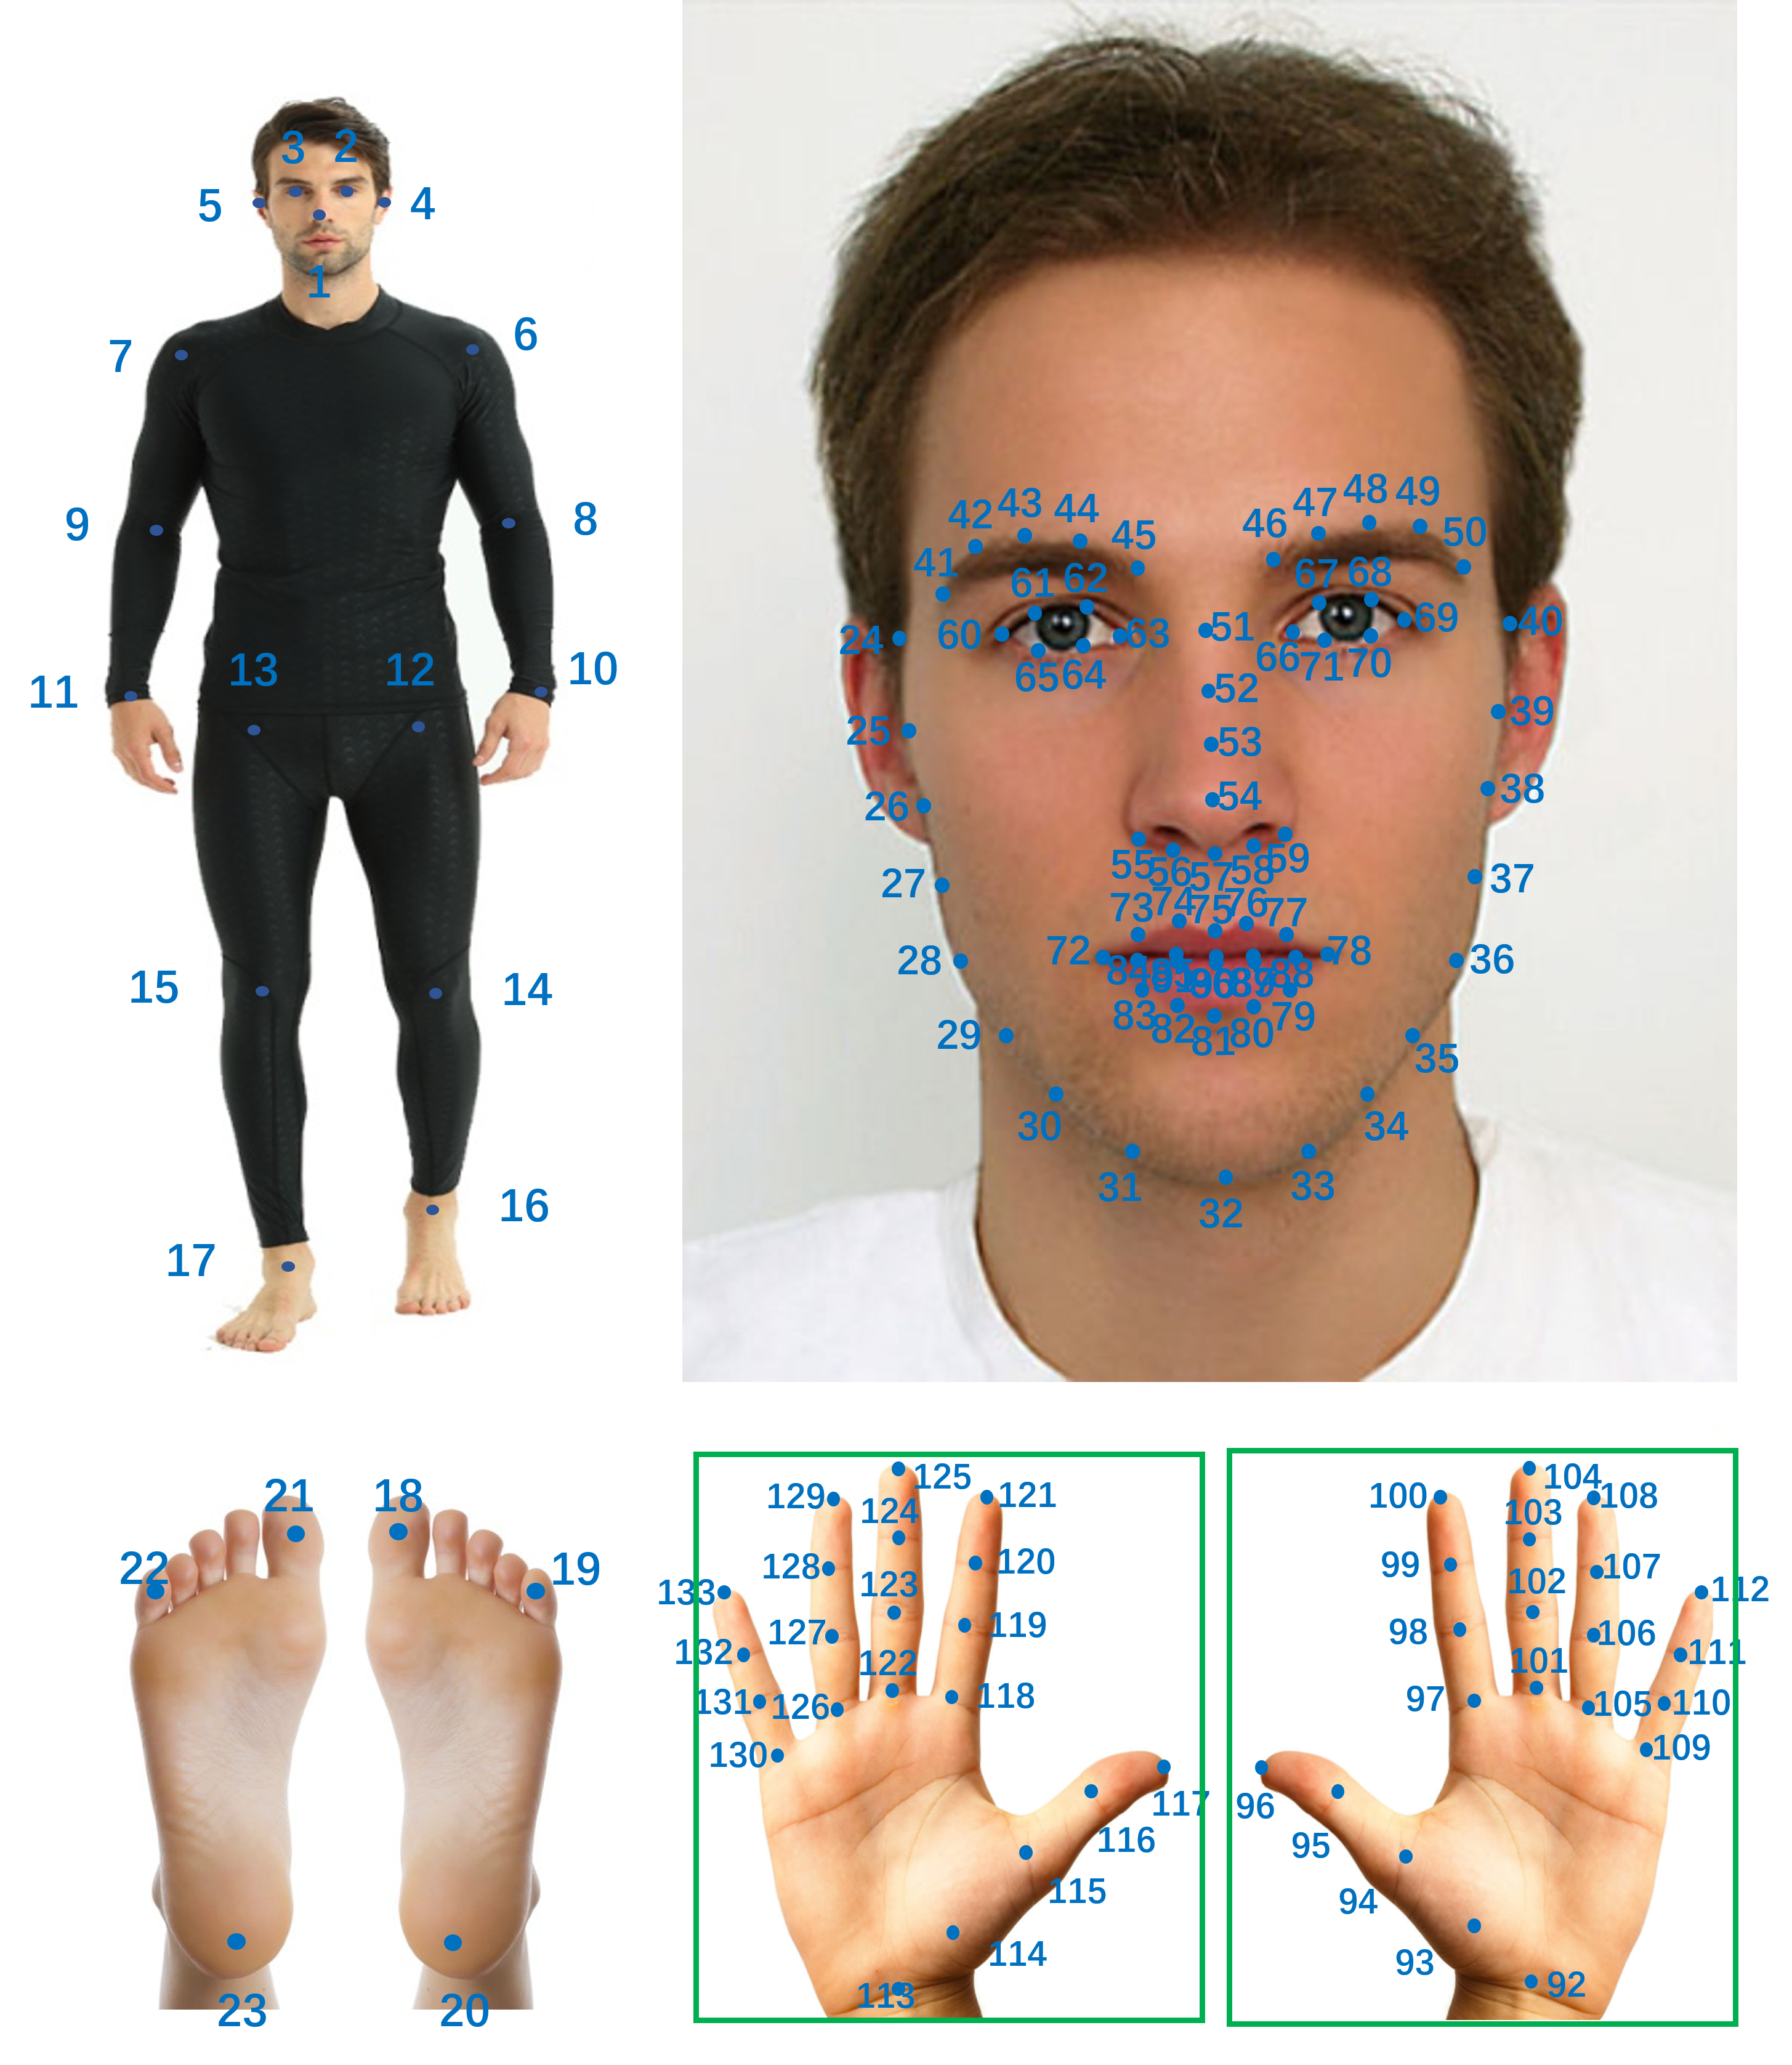
\includegraphics[width=\textwidth]{./m_figures/chapter1/other_model/coco.png}
        \caption{COCO~\cite{coco-wholebody} 格式参考}
        \label{fig:coco}
    \end{subfigure}
    \hfill  % 添加水平间距
    \begin{subfigure}[b]{0.35\textwidth}  % 修改宽度以适应横向排列
        \centering
        \includegraphics[width=\textwidth]{./m_figures/chapter1/other_model/openpose_25.png}
        \caption{Openpose~\cite{openpose} 格式参考}
        \label{fig:openpose}
    \end{subfigure}
    \caption{COCO 和 Openpose 格式参考}
    \label{fig:kp}
\end{figure}


MediaPipe中除了左右手21个关键点,和全身33个关键点的表示之外,对面部有更为详细的定义。
其面部由包括眼球、嘴部等部位在内的478个密集点进行定义,并给出了各点之间构成三角面片的组合关系,使其可进一步重建成网格表示,如图~\ref{fig:mediapipe} 所示。

相较于直接从视频中识别人体关键点,人体各部位均具有很强的结构化信息,可以利用深度学习或统计学方法从人体扫描数据建立基于网格的先验模型,并进一步通过参数控制的方式控制该先验模型,用以表征不同的人体形态和姿态,人体参数化模型表示具有更强的表示能力。
% 1.18 改到这一段
\begin{figure}[!htbp]
    \centering
    \begin{subfigure}[b]{0.9\textwidth}
        \centering
        \includegraphics[width=0.3\textwidth]{./m_figures/chapter1/other_model/m_body.png} \hfill
		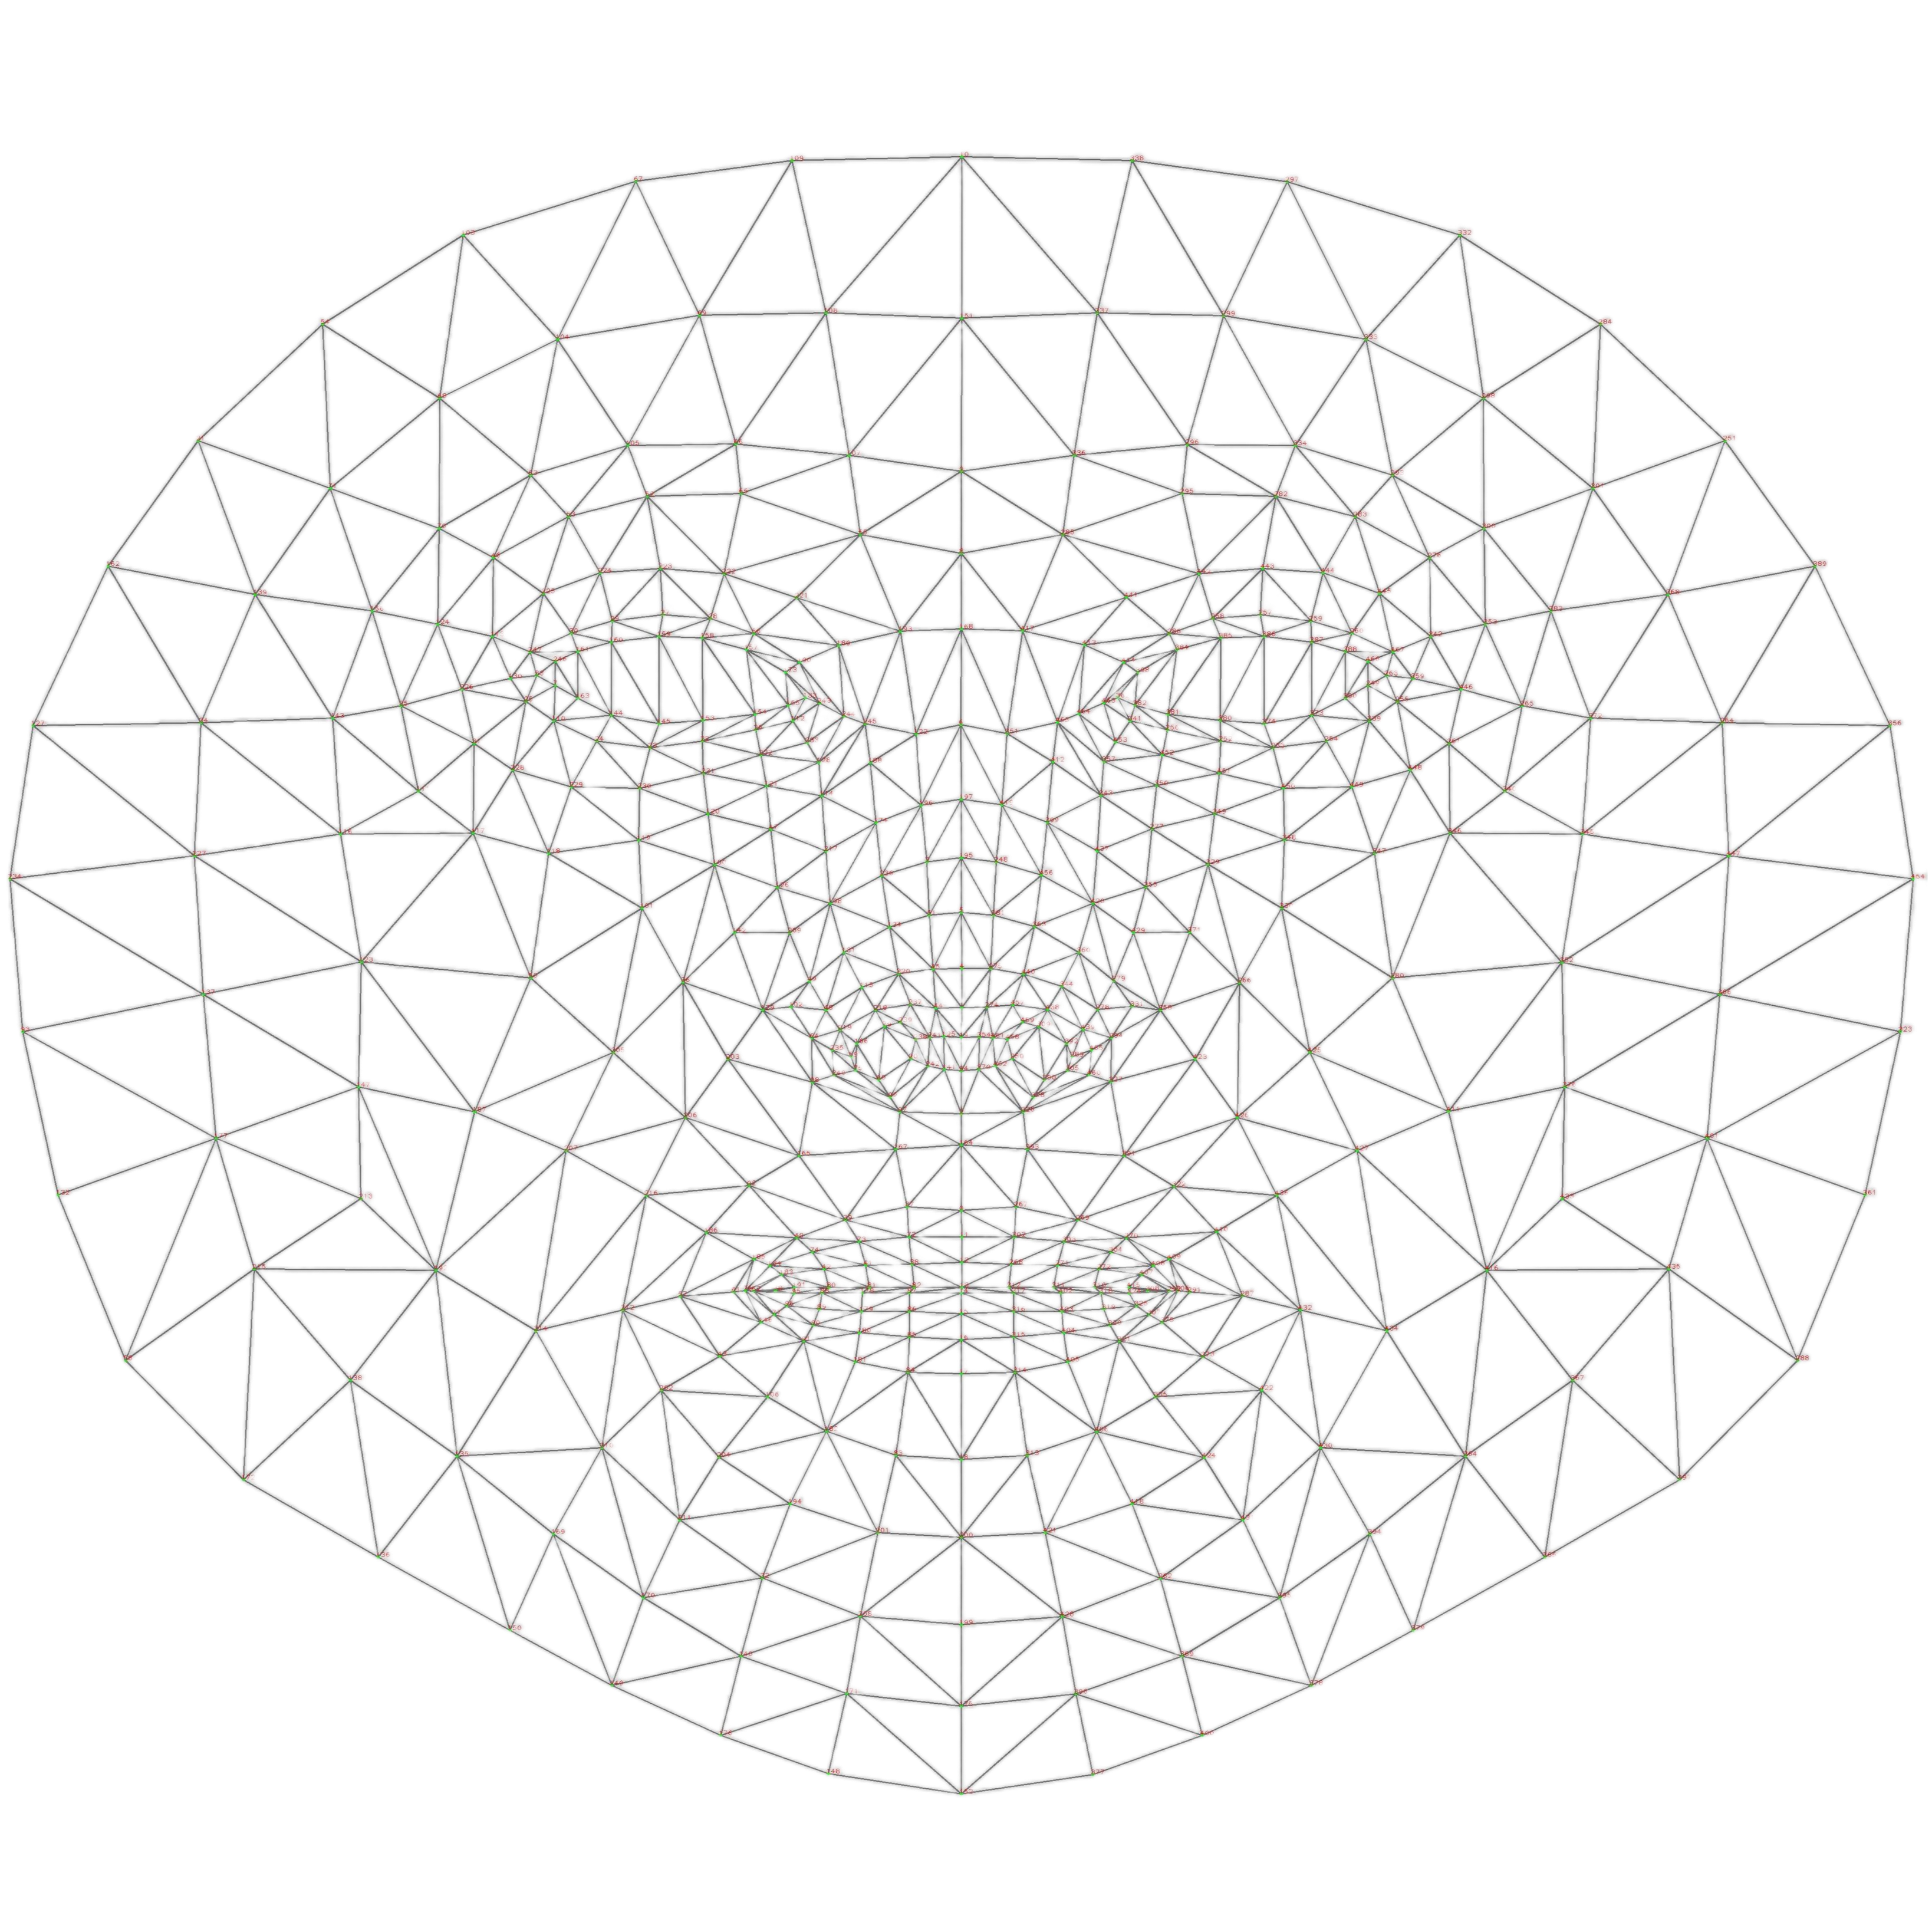
\includegraphics[width=0.3\textwidth]{./m_figures/chapter1/other_model/m_face.png} \hfill
		\includegraphics[width=0.3\textwidth]{./m_figures/chapter1/other_model/m_hand.png}
	\end{subfigure}
	\caption{MediaPipe~\cite{mediapipe} 格式参考}
	\label{fig:mediapipe}
\end{figure}

其中,三维人脸形变模型方法(3D Morphable Face Model,3DMM)\cite{3dmm}首次从三维人脸扫描数据中使用主成分分析方法构建参数化模型。该模型分别使用了表示面部形状和纹理的基向量。通过线性组合这些基向量,模型能够表示不同的三维人脸。一系列衍生方法在 3DMM 模型的基础上进行了拓展和改进,其中 LSFM 方法\cite{lsfm}进一步在模型中分解了人脸表情系数,构建了三维扫描表情数据集;
BFM 方法\cite{bfm}则在人脸模型当中引入了多尺度对称性,能够更细粒度的对人脸的细节变化进行控制;FLAME 方法\cite{FLAME:SiggraphAsia2017}进一步从人脸模型拓展到人头模型,在其中引入了姿态变量,能够进一步对人物头部转动、下颚张合、眼球转动等进行建模;Faceverse \cite{wang2022faceverse} 中利用从 Mediapipe\cite{mediapipe} 检测得到的关键点拟合得到相应的人脸模型系数,进一步提高了拟合速度。图~\ref{fig:3dmm}~展示了部分三维人脸形变模型。

\begin{figure}[!htbp]
    \centering
    \begin{subfigure}[b]{0.5\textwidth}
        \centering
        \includegraphics[height=3cm,width=\textwidth]{./m_figures/chapter1/3dmm/faceverse.jpg}
        \caption{Faceverse~\cite{wang2022faceverse} 模型}
    \end{subfigure}
    \hfill
    \begin{subfigure}[b]{0.45\textwidth}
        \centering
        \includegraphics[width=\textwidth]{./m_figures/chapter1/3dmm/bfm.png}
        \caption{BFM~\cite{bfm} 模型}
    \end{subfigure}
    \vspace{0.5cm}  % 增加竖直间距

	\begin{subfigure}[b]{0.9\textwidth}
        \centering
        \includegraphics[width=\textwidth]{./m_figures/chapter1/3dmm/flame.jpg}
        \caption{FLAME~\cite{FLAME:SiggraphAsia2017} 模型}
    \end{subfigure}
    \caption{各种3DMM模型示例}
    \label{fig:3dmm}
\end{figure}

针对手部的参数化模型最具代表性的工作是 MANO 模型\cite{mano},通过从大规模三维手部扫描数据中建立统计模型,其中基于PCA方法对手部形状建模,基于前向运动学树对手部姿态建模,MANO 模型通过形状参数 $\beta$ 和 姿态参数 $\theta $ 分别控制手部的静态形状和动作姿态。后续的工作如 HTML \cite{qian2020html} 将PCA分解后的纹理表示引入 MANO 模型当中;NIMBLE \cite{li2022nimble} 则结合肌肉和骨骼构建了针对手部的参数化模型。

针对全身的参数化模型,在工作\cite{allen2003space}中,首次将PCA分解应用于表示三维人体形态变化;SCAPE \cite{anguelov2005scape} 中将姿态形变模型引入参数化模型当中,
使得身体模型更具有真实肌肉形变感;在后续的工作\cite{allen2006learning} 则定义了标准线性蒙皮函数来建模姿态相关的形变;而SMPL \cite{smpl} 模型的出现使得参数化人体模型进一步被广泛使用。与 MANO 模型类似,SMPL模型的训练过程主要通过对大量的3D人体扫描数据进行分析,学习形状和姿态之间的关系。为了从3D扫描数据中提取出人体的统计特征,SMPL 也采用了PCA技术,将每个人体的形态表示为形状参数向量,并结合人体的前向运动学树来拟合具体姿势。具体来说,
SMPL\cite{smpl}  网格顶点由如下蒙皮公式(\ref{eq:smplM})控制。
\begin{equation}
    M(\beta, \theta) = W(T_P(\beta, \theta), J(\beta), \theta, W)
    \label{eq:smplM}
\end{equation}

其中,\(W(\cdot)\)表示混合蒙皮公式,\(\beta\)表示人体形状参数,\(\theta\)表示人体姿态参数,\(J(\beta)\)表示模型回归出的关节位置,\(W\)表示混合蒙皮权重。\(T_P(\beta, \theta)\)表示经过体和四肢变形后的人体模型顶点位置,由平均人体模板,形状以及姿态参数混合得到。
后续研究则在SMPL模型的基础上增加了手部、面部等信息,得到了更加生动的身体模型。SMPLH~\cite{smplh} 模型将 MANO 模型与SMPL 模型相结合,使得身体模型能够具有相应的姿态。
SMPLX~\cite{smplx} 在 SMPLH 的基础上进一步引入了 FLAME 模型,将面部动态变化也纳入身体模型当中。图\ref{fig:smpl} 展示了常用的身体模型。
\begin{figure}[!htbp]
    \centering
    \begin{subfigure}[b]{0.35\textwidth}
        \centering
        \includegraphics[width=\textwidth]{./m_figures/chapter1/other_model/smpl.png}
        \caption{SMPL~\cite{smpl} 模型}
    \end{subfigure}
    \hfill
    \begin{subfigure}[b]{0.3\textwidth}
        \centering
        \includegraphics[width=\textwidth]{./m_figures/chapter1/other_model/smplx.png}
        \caption{SMPLX~\cite{smplx} 模型}
    \end{subfigure}
	\hfill
	\begin{subfigure}[b]{0.3\textwidth}
        \centering
        \includegraphics[width=\textwidth]{./m_figures/chapter1/other_model/mano.jpg}
        \caption{MANO~\cite{mano} 模型}
    \end{subfigure}
    \caption{身体模型示例}
    \label{fig:smpl}
\end{figure}

\section{本文主要工作}

综上所述,随着近几年生成式人工智能的高速发展,生成式数字人工作层出不穷,出现了大量的不同的技术方案。但目前生成式数字人作为生成任务的子课题,仍处于探索阶段,目前现有的工作往往从可控性、生成速度、质量、连续性等多个方面探索如何提高生成式数字人的能力,并取得了可观的进展。但是由于人物视频数据的复杂性较高,且包含细粒度标注的视频数据集匮乏,在当前的研究工作中,如下4点局限性依然存在。

1) \textbf{可控性:}生成式数字人需要能够根据输入的动作、文本等多维度数据驱动对应的数字人形象,产生与驱动动作一致,且自然真实的人物视频序列。
然而,部分数字人技术\cite{liu2024anitalker,xu2024hallo}仅局限于单独的人物头像重演,缺乏自然的手势语言交互,缺乏真实感。
部分数字人技术\cite{lin2024cyberhost}仅从音频输入中驱动人物形象,缺乏对人物肢体的控制。
因此为了提高生成式数字人模型对驱动信息的可控性,需要提高驱动模态的有效性和模型对驱动信息的理解能力。

2) \textbf{生成速度:}生成式数字人对于生成速度也存在要求。视频合成实时率用来描述视频合成耗时与输出视频时长比值。
我国《数字虚拟人技术要求》\cite{数字虚拟人技术要求}中要求生成的数字人视频需要不低于25帧每秒,同时在1080分辨率条件下,合成实时率需小于1。
这个要求的提出是因为数字人任务往往需要应用于直播、在线客服等实时领域。而基于扩散模型及 Transformer 架构的生成式数字人模型虽然能够合成高质量的数字人,但其往往需要数十倍于视频时长的生成时间。
难以满足生成式数字人的生成速度要求。同时较长的生成时长也存在明显的产品控制风险,如当进行离线的长时间的数字人节目生成时,冗长的制作周期,使得在制作过程中难以对其中的问题片段进行调整。

3) \textbf{生成质量:}生成式数字人需要能够生成高保真的写实数字人视频序列。
尤其是生成画面细节的丰富度和逼真度。生成式数字人模型最终生成的图像结果不仅需要能够生成嘴部,头部,躯干等主体内容,也需要能够重现眨眼,头发,手部等细微特征的表达,细微表达的缺少会导致生成视频效果呆板,真实性和表现力的下降。

4) \textbf{时序一致性:}生成式数字人需要能够生成具有时序一致性的数字人帧序列。
该连续性包括了数字人动作一致性和视频帧间的一致性。其中动作一致性一般包括人物动作连贯一致,无跳变等方面,而视频一致性则一般包括帧间的过渡效果,画面流畅性等方面。
因此相比于图像生成任务,视频生成任务需要额外考虑帧间的时序建模问题。时序一致性差可能表现为伪影、画面色彩抖动和数字人动作不自然,不规则运动等问题。

因此,本文主要工作围绕生成式数字人领域目前存在的局限性进行研究和改进。提出了基于多维度特征融合的生成式数字人解决方案。首先,本文提出了基于多维度特征的基准数据集构建方法,整合集成了多种关键技术,实现从单目视频数据中提取高质量多维度合成人体数据表征,该合成图像表征能精确的表征数字人的嘴型、眼部、手部及躯体动作,并利于神经网络模型建模。

接着针对该解决方案,以条件式对抗生成网络为基础架构具体实现多维度特征融合的数字人建模。并进一步在该框架下针对数字人生成任务的整体形象和细节表示引入了基于人体大模型的损失函数和基于数字人任务判别器结构优化。从这两个方面实现全局维度特征和局部维度特征的融合。针对生成过程中的时序一致性,本文在当前数字人模型中引入了基于帧间连续特征的时序特征融合方法方法和基于多任务学习的法线特征融合方法。

最后本文整合了驱动与呈现的相关技术方案,以数字人下游实际的应用为例,阐明数字人实际解决方案。利用建模完成的数字人模型,实现了对上述改进方案的验证。

具体来说,本文的主要工作如下:

1) 数字人基准数据集构建方法。该方法从数据的角度出发,解决数字人生成任务中数据匮乏和不一致的问题,提出了一个基于多维度融合的数据集构建流程,整合了多种关键技术,实现了从单目视频数据中提取高质量多维度合成数字人数据样本,构建的合成图像特征能精确的表征数字人的嘴型、眼部、手部及躯体动作,并利于神经网络模型建模。该工作针对性的解决了生成式模型的可控性问题。

2)数字人局部细节和整体形象增强的改进。针对生成式数字人任务,提出基于多维度特征融合的条件对抗生成网络基本架构,该架构能够实时、可控的生成高保真数字人视频。并进一步设计并实现了基于人体大模型的损失函数和基于数字人任务的局部判别器结构。分别从整体形象和局部细节增强数字人建模效果。其中基于条件对抗式生成的模型有效解决了生成速度问题,满足了实时性应用的要求;而针对数字人任务的模型优化则进一步提高了生成质量。

3) 基于帧间连续性和法线约束的时序一致性改进。分别提出基于法线约束的多任务学习方法和基于多帧时序连续性的时序增强方法。前者通过跨帧几何一致性,后者通过连续帧条件约束,均有效提升了生成数字人视频生成的时序一致性。同时结合本文数字人基准数据集构建方法,设计了时序一致性闭环检测方法,用以对生成式数字人视频的时序一致性进行评估。该工作针对时序一致性提出并实现了可行的解决方案,并进一步提出在数字人任务上的时序一致性衡量标准。

4) 基于多维度特征融合的生成式数字人应用案例。本文首先阐明了本文模型在推理驱动阶段时的数据通路,并结合生成式数字人应用案例,进一步阐明了本文所提出的生成式数字人方法如何与其他技术进行结合进行驱动呈现,验证了本文提出的生成式数字人建模方案的可行性。

\section{本文章节安排}

本文章节组织结构如图 \ref{fig:framework} 所示,由如下六个章节组成:
\begin{figure}[!htbp]
	\centering
	\includegraphics[width=0.6\textwidth]{./m_figures/chapter1/框架.pdf}
	\caption{论文结构图}
	\label{fig:framework}
\end{figure}

第 1 章:绪论。该章节介绍了本文的研究背景和研究意义,论述了目前相关的研究工作和数字人生成领域存在的问题,明确了本文主要的工作内容和相关贡献,最后给出文本的结构安排。

第 2 章:生成式数字人中的多维度特征融合总体方案。该章节从宏观的角度概述了本文数字人基于多维度融合的数字人建模方案的总体方案,详细阐述以人为中心的多维度训练集构建流程,并深入分析了本文构建的各模态信息在生成式数字人建模任务的用途。本文构建的合成图像特征能精确的表征数字人的嘴型、眼部、手部及躯体动作,并利于神经网络模型建模。并进一步利用该建模方法构建本文的基准数据集,并针对数字人生成任务,阐明相关的评估指标。

第 3 章:全局人体特征和局部位置特征的融合增强方法。本文以 StyleUNet\cite{styleAvatar} 为实现基准方案,构建了能够融合多维度特征的数字人建模方法。在该框架下针对数字人生成任务的整体形象和细节表示引入了基于人体大模型的损失函数和基于数字人任务的局部判别器结构优化。从这两个方面实现全局维度特征和局部维度特征的融合。

第 4 章:帧间连续性与法线属性融合的时序一致性改进。该章节在上一章实现的基准模型上,分别探索了两条改进路线;即基于法线约束的多任务学习方法和基于连续帧的时序融合方法。分别从几何一致性和帧间时序连续性的两个角度对生成式数字人进行了改进,提升生成数字人视频的时序一致性。最后,本文设计了一套数字人时序一致性闭环检测方法,利用该检测方法,对本章节中的改进在数字人动作时序一致性上进行了评估实验和结果分析,并将最终改进的模型与其他开源模型进行了性能对比。

第 5 章:生成式数字人应用案例。该章节针对数字人驱动呈现任务,首先阐明本文模型在推理时的数据通路,并将建模完成的数字人应用于实际系统当中,进一步阐明了基于本文提出的多维度特征融合的生成式数字人应用方案和具体的交互流程。

第 6 章:总结和展望。该章节对全文工作进行了回顾和总结,提炼了本文的重点工作成果,并对本文工作的局限性及未来可能的改进方向进行了展望。
